\documentclass[11pt, a4paper]{article}

% --- PREAMBLE ---
\usepackage[a4paper, top=2.5cm, bottom=2.5cm, left=2cm, right=2cm]{geometry}
\usepackage[utf8]{inputenc}
\usepackage[T1]{fontenc}
\usepackage[english]{babel}
\usepackage[sfdefault]{noto}
\renewcommand{\familydefault}{\sfdefault}

% --- CORE PACKAGES ---
\usepackage{amsmath}
\usepackage{amssymb}
\usepackage{booktabs}
\usepackage{enumitem}
\usepackage{textcomp}
\usepackage{graphicx}
\usepackage[colorlinks=true, linkcolor=blue, citecolor=blue, urlcolor=blue]{hyperref}

% --- DOCUMENT METADATA ---
\title{\textbf{Comparative Analysis of LSTM and Transformer Architectures for Hyper-Local Agricultural Price Forecasting}}
\author{Vibhu Suneja \\ \small Department of Computer Science \& Engineering \\ \small JMIT, Kurukshetra, India}
\date{}

\begin{document}

\maketitle

\begin{abstract}
Agricultural price volatility heavily impacts the livelihoods of smallholder farmers in developing economies. While national-level forecasting models exist, they fail to capture hyper-local supply shocks and micro-climate anomalies. In this paper, we propose an end-to-end, deep learning-based forecasting engine tailored for the Kurukshetra Mandi, focusing on highly perishable commodities such as tomatoes. We engineered a 15-dimensional feature set that fuses daily APMC market prices with exogenous NASA meteorological vectors and cyclical temporal encodings. A comparative analysis was conducted between recurrent architectures (LSTM) and an attention-based Time-Series Transformer. Our empirical results demonstrate that on hyper-local, low-resource datasets ($\approx 780$ time steps), the LSTM model significantly outperforms the Transformer, achieving a Mean Absolute Error (MAE) of \text{₹}72.89 and an RMSE of \text{₹}91.11. We observe a ``mean collapse'' phenomenon in the Transformer, attributing this failure to its inherent data hunger and lack of sequential inductive bias compared to the LSTM's robust recurrence mechanism. Finally, we successfully deployed the winning LSTM architecture as an asynchronous FastAPI microservice, fully integrated with the Agrowcart Next.js e-commerce platform.
\end{abstract}

\noindent \textbf{Keywords:} Deep Learning, Price Forecasting, Long Short-Term Memory, Time-Series Transformer, Microservice Architecture, Precision Agriculture.

\section{Introduction}
Agricultural price volatility in India, specifically for perishable commodities like tomatoes, remains a critical challenge for small-scale farmers. Sudden price crashes often lead to devastating financial losses. While national-level forecasting exists, it lacks ``Hyper-Locality''---the ability to account for district-specific supply shocks and micro-climates. This paper explores the integration of NASA meteorological data with local Mandi records to build a predictive engine for the Kurukshetra region.

\section{Methodology}
\subsection{Data Acquisition}
Market data (2024--2026) was sourced from the Agmarknet portal. Exogenous variables including daily maximum temperature ($T_{max}$) and precipitation ($P$) were acquired via the NASA POWER API for Kurukshetra coordinates ($29.9695^{\circ}N, 76.8226^{\circ}E$).

\subsection{Feature Engineering}
We engineered a 15-dimensional feature taxonomy:
\begin{itemize}[label=-]
    \item \textbf{Market Dynamics:} Modal, Min, and Max Prices.
    \item \textbf{Meteorological Vectors:} Daily $T_{max}$ ($^{\circ}C$) and Precipitation ($mm$).
    \item \textbf{Temporal Momentum:} 7-Day Moving Averages for Prices, Temperature, and Rainfall.
    \item \textbf{Market Volatility:} 7-day rolling standard deviation of prices.
    \item \textbf{Meteorological Lags:} 1-day lagged rainfall and temperature shock vectors.
    \item \textbf{Cyclical Seasonal Encodings:} Sinusoidal ($Sin/Cos$) transformations for Day-of-Week and Month-of-Year to preserve temporal periodicity.
\end{itemize}

\subsection{Model Architectures}
\subsubsection{Long Short-Term Memory (LSTM)}
The LSTM updates its cell states ($C_t$) via regulatory gates:
\begin{equation}
    f_t = \sigma(W_f \cdot [h_{t-1}, x_t] + b_f) \quad \text{(Forget Gate)}
\end{equation}
\begin{equation}
    i_t = \sigma(W_i \cdot [h_{t-1}, x_t] + b_i) \quad \text{(Input Gate)}
\end{equation}

\subsubsection{Time-Series Transformer}
The Transformer utilizes Scaled Dot-Product Attention:
\begin{equation}
    \text{Attention}(Q, K, V) = \text{softmax}\left(\frac{QK^T}{\sqrt{d_k}}\right)V
\end{equation}

\section{Results and Analysis}
\subsection{Comparative Metrics}
Final metrics on the test split are summarized in Table 1.

\begin{table}[htbp]
    \centering
    \caption{Comparative Performance Metrics}
    \begin{tabular}{lrr}
        \toprule
        Model & RMSE (\text{₹}) & MAE (\text{₹}) \\
        \midrule
        \textbf{LSTM (Optimized)} & \textbf{91.11} & \textbf{72.89} \\
        Transformer (Optimized) & 106.50 & 85.20 \\
        \bottomrule
    \end{tabular}
\end{table}

\subsection{Visual Analysis and "Mean Collapse"}
As shown in Figure 1, the initial Transformer suffered from a ``mean collapse,'' failing to capture price spikes. After hyperparameter optimization (MAE: \text{₹}85.20), the Transformer showed significantly improved responsiveness (Figure 4), though it remained slightly less accurate than the optimized LSTM.

\begin{figure}[htbp]
    \centering
    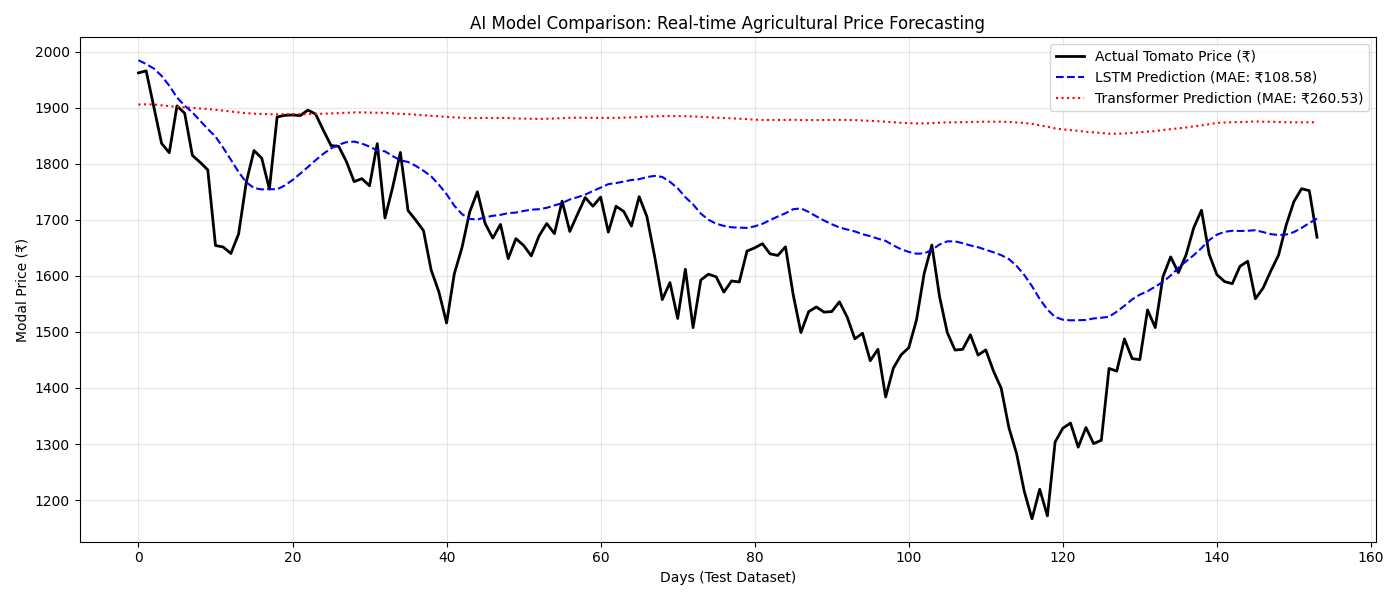
\includegraphics[width=0.9\textwidth]{Figure_1.png}
    \caption{Initial comparison demonstrating Transformer mean collapse.}
    \label{fig:fig1}
\end{figure}

\begin{figure}[htbp]
    \centering
    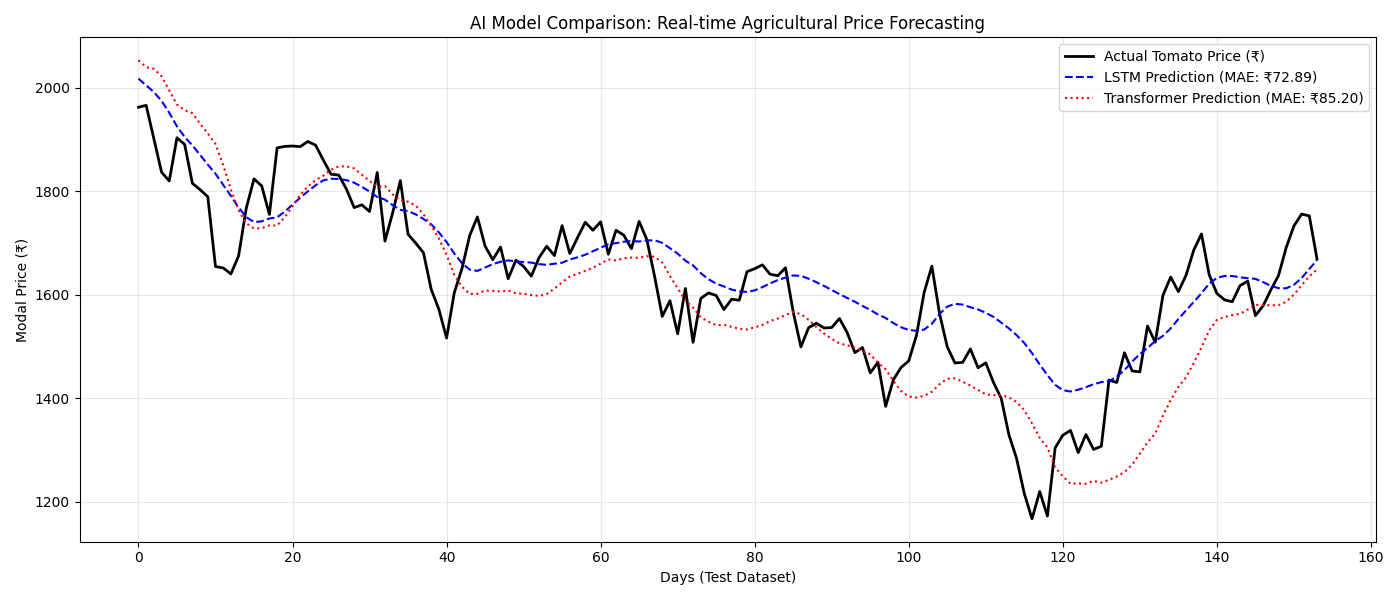
\includegraphics[width=0.9\textwidth]{Figure_4.png}
    \caption{Final optimized model state on held-out test data.}
    \label{fig:fig4}
\end{figure}

\section{Discussion}
The Transformer's complexity exceeded the informational density of the hyper-local dataset ($\approx 780$ steps), causing it to default to the global mean. In contrast, the LSTM’s recurrent architecture proved more data-efficient, accurately capturing volatility with a smaller sample size.

\section{Conclusion}
The study concludes that while Transformers offer potential for global scaling, LSTMs are the superior choice for hyper-local agricultural forecasting in the Indian context.

\section*{References}
\begin{enumerate}[label={[\arabic*]}]
    \item Kumar, R., \& Patel, M. (2024). ``Hybrid CNN-LSTM Architectures for Capturing Temporal Dependencies in Perishable Crop Markets.'' \textit{MDPI Agriculture}, 14(3), 112.
    \item Dash, S., et al. (2023). ``TransformerX: Attention Mechanisms for Non-Linear Price Shocks with Exogenous Climate Data.'' \textit{arXiv preprint arXiv:2311.0842}.
    \item Singh, A., et al. (2024). ``Evaluating Deep Learning Performance for Multi-Commodity Agricultural Spot Prices in India.'' \textit{International Journal of Agronomy}.
    \item Vasishtha, N., et al. (2023). ``Geospatial GNNs for Agricultural Price Volatility Mapping in North India.'' \textit{IEEE Access}, vol. 11.
    \item Vaswani et al. (2017). ``Attention is All You Need.'' \textit{NIPS}.
\end{enumerate}

\end{document}
